\chapter{Introduction into time-series analysis.}
The time-series is a data type represented by a sequence of datapoints sampled at successive times and usually found as the sequence of real or integer numbers with attached timestamps. 
The time-series data is arising naturally from observations and reflecting an evolution of some subject or a development of some phenomena in time. It is very common to see the financial information like stocks or currency fluctuations presented through the means of the visualized time-series on the TV or in newspapers. The medical observations such as a blood pressure or a body temperature fluctuations is another example of a time-series commonly seen in life. According to Tufte \cite{citeulike:1454223} ``The time-series plot is the most frequently used form of graphic design. With one dimension marching along to the regular rhythm of seconds, minutes, hours, days, weeks, months, years, or millennia, the natural ordering of the time scale gives this design a strength and efficiency of interpretation found in no other graphic arrangement.'' The figure \ref{fig:10century} from the Tufte book depicts the oldest known example of a time-series plot showing the planetary orbits inclinations and is dated by tenth century.

\begin{figure}[tbp]
   \centering
   \includegraphics[height=70mm]{figures/10century.eps}
   %%{seriesheatmap}
   \caption{Ancient time-series plot showing the planetary orbits inclinations.}
   \label{fig:10century}
\end{figure} 

It is generally assumed that the consecutive measured values stored in the time-series are sampled at equally spaced time intervals.
This specific ordering of samples in time often bear the temporal information about the dependency of successive observation on earlier ones and the explicit recognition of such ordering is a key feature which distinguishes the time-series data from usually independent statistical samples and makes the time-series analysis techniques somehow different from statistical analyses \cite{citeulike:3989988}. 

The time-series analysis methods in general combine various statistical and pattern recognition approaches while using temporal information presented from the ordering of samples. Historically time-series analysis is divided by two major fields of study: first is the explorative and descriptive analysis and the second field is the forecasting. 

While the descriptive analyses focused on the understanding of the time-series generating processes itself by finding seasonal trends, periodicity or some hidden features within the time-series, the predictive analyses aiming forecasting the future of the time-series generating process based on the information found by conducting descriptive analyses \cite{citeulike:3449765}. Nevertheless, both, descriptive and predictive analyses, based on the identification of some pattern in the time-series which could be formally described and correspond to the time-series generating process nature. Once this pattern is found and compiled into the formal model during the explorative analysis it is used for the extrapolation of the time-series into future. Such a model development and forecasting started probably from the babylonian astrologists predicting celestial phenomenas and novadays scientists are using stochastic and deterministic models based on the timeseries analysis in almost every scientific field.